\chapter{提案手法}\label{abst}
本章では,座り方による個人認証を行うための手法について詳しく述べる.

\section{提案手法の概要}
本研究では,本人と本人以外の2クラスに分類することを目的としている.
そのため,2クラスのパターン認識において高い認証性能を持つSVMを用いる.

Kinectを用いて関節位置の3次元座標を取得し,前処理,特徴抽出を行った後,SVMを使用して2クラスに分類し認証を行う.

また,未学習データに対する性能を向上させるための工夫がされていることもSVMを用いる理由である.
以下では,それぞれの処理の流れについて詳しく述べる.

\section{提案手法の流れ}
提案手法の流れを図\ref{fig:syuho}に示す.まず,Kinectを用いて骨格情報を取得する.次に,前処理として,
Kinectから取得した3次元座標を相対座標に変換する.骨格座標の座標軸は,図3.2に示すように,
Kinectの赤外線カメラを中心に右手座標系である.つまり,赤外線カメラの位置を原点としている.
そのため,初期位置に多少のずれがある場合,正確な特徴抽出を行うことが難しい.そこで,
前処理として背骨の座標を原点とした相対座標への変換を行う.
全ての関節位置の座標から背骨の座標を引くことにより相対座標へ変換する.これにより,初期位置のずれに頑健になり,
より正確な骨格の特徴を取得することが可能になる.

\newpage

\begin{figure}[htbp]
  \begin{center}
    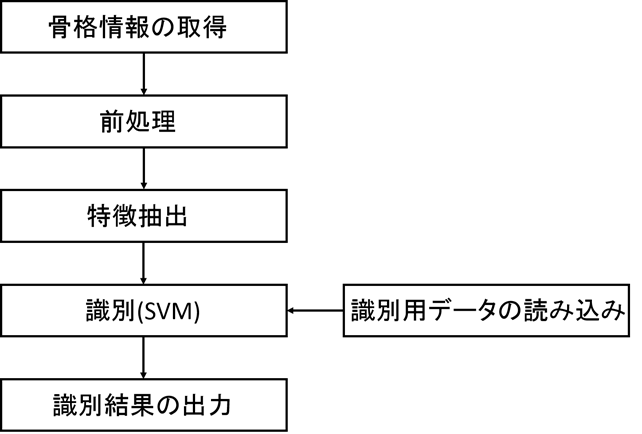
\includegraphics[clip,width=7.0cm]{./images/nagare.png}
    \caption{提案手法の流れ}
    \label{fig:syuho}
  \end{center}
\end{figure}

\begin{figure}[htbp]
  \begin{center}
    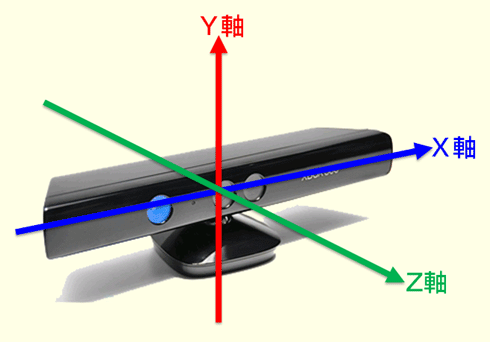
\includegraphics[clip,width=7.0cm]{./images/zahyo.png}
    \caption{骨格座標系}
    \label{fig:zahyo}
  \end{center}
\end{figure}

前処理を行った座標を,0.5秒ごとに平均を計算することで特徴抽出を行う.座る動作には,歩く動作など複数の動作が合わさることが多い.
また,人それぞれ座る速度も異なる.一定時間で分割することで,そういった特徴をより多く抽出することが可能になる.
そして,得られた特徴からSVMを用いて識別を行い,認証結果を出力する.